\documentclass[psamsfonts]{amsart}
%
%-------Packages---------
%
\usepackage[h margin=1 in, v margin=1 in]{geometry}
\usepackage{amssymb,amsfonts}
\usepackage{rank-2-roots}
\usepackage[all,arc]{xy}
\usepackage{tikz-cd}
\usepackage{enumerate}
\usepackage{mathrsfs}
\usepackage{amsthm}
\usepackage{mathpazo}
\usepackage{yfonts}
\usepackage{enumitem}
\usepackage{mathrsfs}
\usepackage{fourier-orns}
\usepackage[all]{xy}
\usepackage{hyperref}
\usepackage{cite}
\usepackage{url}
\usepackage{mathtools}
\usepackage{graphicx}
\usepackage{pdfsync}
\usepackage{mathdots}
\usepackage{calligra}
%
\usepackage{tgpagella}
\usepackage[T1]{fontenc}
%
\usepackage{listings}
\usepackage{color}

\definecolor{dkgreen}{rgb}{0,0.6,0}
\definecolor{gray}{rgb}{0.5,0.5,0.5}
\definecolor{mauve}{rgb}{0.58,0,0.82}

\lstset{frame=tb,
  language=Matlab,
  aboveskip=3mm,
  belowskip=3mm,
  showstringspaces=false,
  columns=flexible,
  basicstyle={\small\ttfamily},
  numbers=none,
  numberstyle=\tiny\color{gray},
  keywordstyle=\color{blue},
  commentstyle=\color{dkgreen},
  stringstyle=\color{mauve},
  breaklines=true,
  breakatwhitespace=true,
  tabsize=3
  }
%
%--------Theorem Environments--------
%
\newtheorem{thm}{Theorem}[section]
\newtheorem*{thm*}{Theorem}
\newtheorem{cor}[thm]{Corollary}
\newtheorem{prop}[thm]{Proposition}
\newtheorem{lem}[thm]{Lemma}
\newtheorem*{lem*}{Lemma}
\newtheorem{conj}[thm]{Conjecture}
\newtheorem{quest}[thm]{Question}
%
\theoremstyle{definition}
\newtheorem{defn}[thm]{Definition}
\newtheorem*{defn*}{Definition}
\newtheorem{defns}[thm]{Definitions}
\newtheorem{con}[thm]{Construction}
\newtheorem{exmp}[thm]{Example}
\newtheorem{exmps}[thm]{Examples}
\newtheorem{notn}[thm]{Notation}
\newtheorem{notns}[thm]{Notations}
\newtheorem{addm}[thm]{Addendum}
\newtheorem{exer}[thm]{Exercise}
%
\theoremstyle{remark}
\newtheorem{rem}[thm]{Remark}
\newtheorem*{claim}{Claim}
\newtheorem*{aside*}{Aside}
\newtheorem*{rem*}{Remark}
\newtheorem*{hint*}{Hint}
\newtheorem*{note}{Note}
\newtheorem{rems}[thm]{Remarks}
\newtheorem{warn}[thm]{Warning}
\newtheorem{sch}[thm]{Scholium}
%
%--------Macros--------
\renewcommand{\qedsymbol}{$\blacksquare$}
\renewcommand{\sl}{\mathfrak{sl}}
\renewcommand{\hom}{\mathsf{Hom}}
\renewcommand{\emptyset}{\varnothing}
\renewcommand{\O}{\mathscr{O}}
\newcommand{\R}{\mathbb{R}}
\newcommand{\ib}[1]{\textbf{\textit{#1}}}
\newcommand{\Q}{\mathbb{Q}}
\newcommand{\Z}{\mathbb{Z}}
\newcommand{\N}{\mathbb{N}}
\newcommand{\C}{\mathbb{C}}
\newcommand{\A}{\mathbb{A}}
\newcommand{\F}{\mathbb{F}}
\newcommand{\M}{\mathcal{M}}
\renewcommand{\S}{\mathbb{S}}
\newcommand{\V}{\vec{v}}
\newcommand{\RP}{\mathbb{RP}}
\newcommand{\CP}{\mathbb{CP}}
\newcommand{\B}{\mathcal{B}}
\newcommand{\GL}{\mathsf{GL}}
\newcommand{\SL}{\mathsf{SL}}
\newcommand{\SP}{\mathsf{SP}}
\newcommand{\SO}{\mathsf{SO}}
\newcommand{\SU}{\mathsf{SU}}
\newcommand{\gl}{\mathfrak{gl}}
\newcommand{\g}{\mathfrak{g}}
\newcommand{\h}{\mathfrak{h}}
\newcommand{\inv}{^{-1}}
\newcommand{\bra}[2]{ \left[ #1, #2 \right] }
\newcommand{\set}[1]{\left\lbrace #1 \right\rbrace}
\newcommand{\abs}[1]{\left\lvert#1\right\rvert}
\newcommand{\norm}[1]{\left\lVert#1\right\rVert}
\newcommand{\transv}{\mathrel{\text{\tpitchfork}}}
\newcommand{\enumbreak}{\ \\ \vspace{-\baselineskip}}
\let\oldexists\exists
\renewcommand\exists{\oldexists~}
\let\oldL\L
\renewcommand\L{\mathfrak{L}}
\makeatletter
\newcommand{\tpitchfork}{%
  \vbox{
    \baselineskip\z@skip
    \lineskip-.52ex
    \lineskiplimit\maxdimen
    \m@th
    \ialign{##\crcr\hidewidth\smash{$-$}\hidewidth\crcr$\pitchfork$\crcr}
  }%
}
\makeatother
\newcommand{\bd}{\partial}
\newcommand{\lang}{\begin{picture}(5,7)
\put(1.1,2.5){\rotatebox{45}{\line(1,0){6.0}}}
\put(1.1,2.5){\rotatebox{315}{\line(1,0){6.0}}}
\end{picture}}
\newcommand{\rang}{\begin{picture}(5,7)
\put(.1,2.5){\rotatebox{135}{\line(1,0){6.0}}}
\put(.1,2.5){\rotatebox{225}{\line(1,0){6.0}}}
\end{picture}}
\DeclareMathOperator{\id}{id}
\DeclareMathOperator{\im}{Im}
\DeclareMathOperator{\codim}{codim}
\DeclareMathOperator{\coker}{coker}
\DeclareMathOperator{\supp}{supp}
\DeclareMathOperator{\inter}{Int}
\DeclareMathOperator{\sign}{sign}
\DeclareMathOperator{\sgn}{sgn}
\DeclareMathOperator{\indx}{ind}
\DeclareMathOperator{\alt}{Alt}
\DeclareMathOperator{\Aut}{Aut}
\DeclareMathOperator{\trace}{trace}
\DeclareMathOperator{\ad}{ad}
\DeclareMathOperator{\End}{End}
\DeclareMathOperator{\Ad}{Ad}
\DeclareMathOperator{\Lie}{Lie}
\DeclareMathOperator{\spn}{span}
\DeclareMathOperator{\dv}{div}
\DeclareMathOperator{\grad}{grad}
\DeclareMathOperator{\Sym}{Sym}
\DeclareMathOperator{\sheafhom}{\mathscr{H}\text{\kern -3pt {\calligra\large om}}\,}
\newcommand*\myhrulefill{%
   \leavevmode\leaders\hrule depth-2pt height 2.4pt\hfill\kern0pt}
\newcommand\niceending[1]{%
  \begin{center}%
    \LARGE \myhrulefill \hspace{0.2cm} #1 \hspace{0.2cm} \myhrulefill%
  \end{center}}
\newcommand*\sectionend{\niceending{\decofourleft\decofourright}}
\newcommand*\subsectionend{\niceending{\decosix}}
\def\upint{\mathchoice%
    {\mkern13mu\overline{\vphantom{\intop}\mkern7mu}\mkern-20mu}%
    {\mkern7mu\overline{\vphantom{\intop}\mkern7mu}\mkern-14mu}%
    {\mkern7mu\overline{\vphantom{\intop}\mkern7mu}\mkern-14mu}%
    {\mkern7mu\overline{\vphantom{\intop}\mkern7mu}\mkern-14mu}%
  \int}
\def\lowint{\mkern3mu\underline{\vphantom{\intop}\mkern7mu}\mkern-10mu\int}
%
%--------Hypersetup--------
%
\hypersetup{
    colorlinks,
    citecolor=black,
    filecolor=black,
    linkcolor=blue,
    urlcolor=blacksquare
}
%
%--------Solution--------
%
\newenvironment{solution}
  {\begin{proof}[Solution]}
  {\end{proof}}
%
%--------Graphics--------
%
%\graphicspath{ {images/} }

\begin{document}
%
\author{Jeffrey Jiang}
%
\title{Representations of $\sl_3\C$}
%
\setcounter{section}{1}
%
\maketitle
%
The representation theory of $\sl_3\C$ is more complex than the situation with
$\sl_2\C$, and involves generalizing some of the tools used to analyze the
irreducible representations of $\sl_2\C$. However, this will develop a
relatively general framework for understanding the representations of
semisimple Lie algebras.\\

Recall that the key piece for understanding the irreducible representations of
$\sl_2\C$ was the basis $H$, $X$, and $Y$, where $H$ was diagonzlizable and
satisfied the commutation relations
\[
[H,X] = 2X \qquad [H,Y] = -2Y \qquad [X,Y] = H
\]

for the higher dimensional case, we will not have such a basis anymore. The idea
will be to replace the matrix $H$ with an abelian subalgebra $\h$. The reasoning
here is that commuting matrices preserve each other's eigenspaces, so they
are simultaneously diagonalizable.
%
\begin{defn}
Given a representation $V$ and a subalgebra $\h \subset \sl_3\C$, a vector
$v \in V$ is an \ib{eigenvector} for $\h$ if for all $H \in \h$, $v$ is an
eigenvector for $H$.
\end{defn}
%
Note that the eigenvalues for a eigenvector $v$ need not be the same for different
$H$. Instead, we have that $Hv = \lambda(H)v$ for some $\lambda \in \h^*$.
Therefore, the generalization of the eigenspace decomposition for an representation
of $\sl_2\C$ is a decomposition $V = \oplus_\lambda V_\lambda$ where $\lambda$
ranges over a finite subset of $\h^*$. We also want to generalize the commutation
relations from $\sl_2\C$. We see that from before, $X$ and $Y$ are eigenvectors
of $\ad(H)$, with eigenvalues $2$ and $-2$ repsectively. When we replace $H$ with
$\h$, we see we want to find a decomposition of $\sl_3\C$ as
\[
\sl_3\C = \h \oplus(\bigoplus_\alpha V_\alpha)
\]
where each $V_\alpha$ is an eigenspace for $\ad(\h)$, and again, the $\alpha$ form
a finite subset of $\h^*$. This procedure will also be used in the general case
as well. \\

When we specialize to $\sl_3\C$, it turns out that an ideal choice of $\h$ is
the subalgebra of diagonal matrices in $\sl_3\C$. Let $L_i$ denote the linear
functionals such that $L_i(A) = A^i_i$. Then the condition that the matrices
in $\sl_3\C$ are traceless implies the dual $\h^*$ is given by linear
combinations $a^iL_i$ where we quotient by the relation $L_1 + L_2 + L_3 = 0$.
We then want to find eigenvectors of $\ad(\h)$. To do this, let $D$ denote
an arbitrary diagonal matrix in $\h$, and $M \in \sl_3\C$. Then $DM$ is the
matrix where $(DM)^i_j = D^i_iM^i_j$ (i.e. the $i^{th}$ row is multiplied by
$D^i_i$), and $MD$ is the matrix where $(MD)^i_j = D^j_jM^i_j$ (i.e. the $j^{th}$
column of $MD$ is multiplied by $D^j_j$). Therefore, the $(i,j)^{th}$ component
of the commutator $[D,M]^i_j$ is given by
\[
[D,M]^i_j = (DM)^i_j - (MD)^i_j = D^i_iM^i_j - D^j_jM^i_j = (D^i_i - D^j_j)M^i_j
\]
Therefore, for a matrix to be and eigenvector of $\ad(D)$ for all $D \in \h$, we
need all but a single entry to be $0$. To see this, we note that we can pick
a matrix $D$ such that the multipliers $(D^i_i = D^j_j)$ for the $M^i_j$
component are all different, so $M$ can only be an eigenvector for $\ad(D)$
if all but one of the entries is $0$. Then the elementary matrices $E_{ij}$ with
a $1$ in the $(i,j)$ give an eigenspace decomposition for $\sl_3\C$, and the
action of $\ad(D)$ on $E_{ij}$ will have eigenvalue $L_i(D) - L_j(D)$. This gives
us that the eigenspace generated by $E_{ij}$ will have ``eigenvalue"
$L_i - L_j \in \h^*$.
%
\iffalse
\center
\scalebox{3}{
  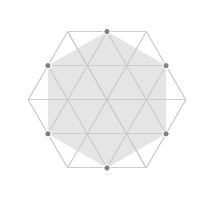
\begin{tikzpicture}[baseline=-.5]
  \begin{rootSystem}{A}
  \roots
  \end{rootSystem}
  \end{tikzpicture}
}
\fi
%
\end{document}
